\documentclass[11pt]{article}
\usepackage[letterpaper,margin=1in]{geometry}
\usepackage{amsmath,amssymb,amsthm}
\usepackage{lmodern}
\usepackage[T1]{fontenc}
\usepackage[utf8]{inputenc}
\usepackage{booktabs}
\usepackage{graphicx}
\usepackage{array}
\usepackage{enumitem}
\usepackage{xcolor}
\usepackage[colorlinks=true,linkcolor=blue!45!black,citecolor=blue!45!black,urlcolor=blue!45!black,pdfpagemode=UseNone]{hyperref}

\hypersetup{
  pdftitle={A geometric characterization of the standard MOND interpolating function},
  pdfauthor={J. Pablo Figueroa Torres},
  pdfsubject={Modified Newtonian Dynamics (MOND); interpolating function; isotropy},
  pdfkeywords={MOND; interpolating function; isotropy; solid angle; emergent gravity; radial acceleration relation; baryonic Tully-Fisher relation}
}

\newtheorem{axiom}{Axiom}
\newtheorem*{theorem*}{Theorem}
\theoremstyle{plain}

\setlength{\parindent}{1.2em}
\setlength{\parskip}{0.2em}

\title{\vspace{-2em}A geometric characterization of the standard MOND interpolating function:\\[2pt]
$\mu(x) = x/\sqrt{1+x^2}$ as the isotropic distribution of $\cot\theta$}
\author{J.\ Pablo Figueroa Torres\\[2pt]
\normalsize Independent Researcher --- \href{https://orcid.org/0009-0005-5297-8777}{ORCID: 0009-0005-5297-8777}}
\date{July 2026 --- v3}

\begin{document}
\maketitle
\vspace{-1.5em}

\noindent\textbf{Abstract.} The interpolating function $\mu(x)$ of Modified Newtonian Dynamics (MOND) phenomenology has been chosen empirically for four decades; standard reviews state explicitly that no derivation from first principles exists. We point out an exact identity: the standard interpolating function, $\mu(x) = x/\sqrt{1+x^2}$, is the cumulative distribution of $\cot\theta$ for directions distributed isotropically on the hemisphere --- equivalently, the threshold density it implies, $\mu'(\Lambda_c) = (1+\Lambda_c^2)^{-3/2}$, is exactly the isotropic probability density of the ratio of longitudinal to transverse field projections. Operationally, $\mu(x)$ is the solid-angle fraction of channels activated by the tilt criterion $|\mathbf{g}\times\hat n| > a_0|\hat n\cdot\hat g|$: misalignment with the local field beyond $\arctan(a_0/g)$. The statement is elementary spherical geometry with no free parameters; $a_0$ enters only as the unit of the threshold. We delimit the content precisely: any monotone interpolating function is \emph{some} solid-angle fraction (the correspondence gate $\leftrightarrow$ $\mu$ is one-to-one), so the specificity of the standard $\mu$ is that its threshold variable is the canonical projection ratio $\cot\theta$, and its gate is a linear comparison of field projections --- the only such gate among the simple projection criteria (tilt, magnitude, longitudinal, perpendicular) with the correct MOND limits, and the one that rigidly fixes the member $\alpha=2$ of the empirical family $\mu_\alpha = x/(1+x^\alpha)^{1/\alpha}$. As corollaries, the flow function $\beta(\Phi) = -\Phi(2+\Phi)(1+\Phi)/[2+\Phi(2+\Phi)]$ follows exactly, with attractor slope $\beta'(0)=-1$ and curvature $\kappa=1/2$, making the baryonic Tully--Fisher relation a dynamical attractor. A Monte Carlo over $10^7$ hard gates reproduces $\beta'(0)=-0.99$, $\kappa=0.47$ with no tuning. We then show that the same flow supplies a model-independent exclusion criterion. Expanding any interpolating function as $\mu = x + c_2x^2 + c_3x^3 + \dots$, the flow is analytic at the Tully--Fisher fixed point if and only if $c_2=0$; the criterion is invariant under the choice of acceleration unit and uses neither axiom. Three widely used forms --- the simple function, the TeVeS toy function and $1-e^{-x}$ --- fail it: their flow is not Lipschitz at the fixed point, so the Tully--Fisher departure reaches zero at \emph{finite} flow time, and a population with a spread of departures is predicted to become \emph{bimodal} at $z\gtrsim1$ rather than merely narrower. That signature forms if and only if the flow is non-Lipschitz, and is therefore not reproducible by tuning parameters within an analytic flow. All symbolic and numerical results are reproducible from the scripts archived with this letter.

\medskip
\noindent\textbf{Keywords:} MOND; interpolating function; isotropy; solid angle; emergent gravity; radial acceleration relation; baryonic Tully--Fisher relation

\section{Introduction}\label{sec:intro}

MOND phenomenology [Milgrom 1983a,b,c] accounts for galactic rotation curves through a relation $\mu(g/a_0)\,\mathbf{g} = \mathbf{g}_N$ (or its inverted form), where the interpolating function $\mu(x)$ satisfies $\mu\to x$ for $x\ll 1$ and $\mu\to 1$ for $x\gg 1$, and $a_0 \simeq 1.2\times10^{-10}\ \mathrm{m\,s^{-2}}$. The functional form of $\mu$ has always been an empirical input: Milgrom (1983a) proposed the simple ($x/(1+x)$) and standard ($x/\sqrt{1+x^2}$) forms as convenient examples; AQUAL [Bekenstein \& Milgrom 1984] requires only the asymptotic limits; and the Living Review by Famaey \& McGaugh (2012) states that no derivation of $\mu$ from first principles is available. The radial-acceleration relation [McGaugh, Lelli \& Schombert 2016a] measured on the SPARC sample [Lelli, McGaugh \& Schombert 2016b] has sharpened the empirical constraints on $\mu$ without changing its status as an ansatz.

This letter proves an elementary identity which, to our knowledge, has not appeared in the literature: \textbf{the standard interpolating function is the cumulative distribution of $\cot\theta$ under isotropy.} If gravitational ``channels'' are distributed isotropically in direction and a channel is active precisely when its misalignment with the local field exceeds a critical tilt $\arctan(a_0/g)$, then the active fraction is $\mu(x)=x/\sqrt{1+x^2}$ with $x=g/a_0$, exactly. No parameter is adjusted; the computation is a one-line integral over a spherical cap. We are equally explicit about what is \emph{not} special: any monotone interpolating function can be written as a solid-angle fraction under some angular gate, because the correspondence between monotone gates and monotone $\mu$'s is one-to-one (\S\ref{sec:uniqueness}). The non-trivial content is \emph{which} threshold variable the standard function singles out --- the ratio of longitudinal to transverse projections, $\cot\theta$, the canonical dimensionless coordinate of a direction relative to the field --- and that the corresponding gate is a linear comparison of field projections, unlike the gates implied by the other members of the empirical $\mu_\alpha$ family.

We emphasize the scope honestly. The theorem is purely geometric: it converts the choice of $\mu$ into the choice of an activation criterion, and shows that criterion to be uniquely selective within a natural class. The physical origin of the tilt criterion --- why dissipation competes in precisely this projection --- is a separate dynamical question that we take up in a forthcoming companion paper, building on the emergent-gravity framework already presented in [Figueroa Torres 2026]; it is not required for any statement made here. Likewise, the value of $a_0$ is not derived here; it enters only as the unit of the threshold.

\section{Axioms and theorem}\label{sec:theorem}

Let $\mathbf{g}$ be the local gravitational field, $g=|\mathbf{g}|$, $x\equiv g/a_0$, and let $\hat n$ denote the direction of a channel (the microscopic degree of freedom whose activation is at stake; its nature is not needed for the theorem).

\begin{axiom}[isotropy]
Channels carry unoriented directions (axes): $\hat n$ and $-\hat n$ label the same channel. The space of channel directions is therefore the hemisphere $\hat n\cdot\hat g\geq 0$ --- not half of the possibilities but all of them --- with the rotation-invariant (Haar) measure $\sin\theta\,d\theta\,d\phi$, where $\theta\in[0,\pi/2]$ is the angle between $\hat n$ and $\hat g$. (Equivalently, on the full sphere the criterion below is written with $|\hat n\cdot\hat g|$ and every statement is unchanged.)
\end{axiom}

\begin{axiom}[tilt activation]
A channel is active if and only if
\begin{equation*}\tag{1}\label{eq:1}
|\mathbf{g}\times\hat n| > a_0|\hat n\cdot\hat g|,
\end{equation*}
equivalently $g\sin\theta > a_0\cos\theta$, i.e., misalignment beyond the critical cone
\begin{equation*}\tag{2}\label{eq:2}
\theta_0(x) = \arctan(1/x).
\end{equation*}
\end{axiom}

\begin{theorem*}
Under Axioms 1--2, the active fraction of channels is
\begin{equation*}\tag{3}\label{eq:3}
\mu(x) = \frac{\Omega_{\text{active}}}{\Omega_{\text{total}}} = \int_{\arctan(1/x)}^{\pi/2}\sin\theta\,d\theta = \cos\big(\arctan(1/x)\big) = \frac{x}{\sqrt{1+x^2}}.
\end{equation*}
\end{theorem*}

\begin{proof}
The measure of Axiom 1 normalizes to $\int_0^{\pi/2}\sin\theta\,d\theta=1$ on the hemisphere ($\phi$ integrates out). Axiom 2 activates the band $\theta>\theta_0$, whose measure is $\cos\theta_0$ --- the complement of the spherical cap of half-angle $\theta_0$. With $\theta_0=\arctan(1/x)$, $\cos\theta_0 = x/\sqrt{1+x^2}$.
\end{proof}

Both MOND limits are immediate, and the small-$x$ expansion is
\begin{equation*}\tag{4}\label{eq:4}
\mu(x) = x - \tfrac12 x^3 + \mathcal{O}(x^5), \qquad \mu(x\to\infty)\to 1.
\end{equation*}

Two remarks. (i) At $g=a_0$ the critical cone is exactly $45^\circ$: the acceleration scale marks the tilt at which alignment and misalignment are balanced. (ii) \textbf{The central identity.} Equivalently, $\mu(x)$ is the fraction of solid angle with $\cot\theta < x$, and the threshold density it implies is
\begin{equation*}\tag{5}\label{eq:5}
P(\Lambda_c) = \mu'(\Lambda_c) = (1+\Lambda_c^2)^{-3/2}, \qquad \int_0^\infty P\,d\Lambda_c = 1,
\end{equation*}
which is exactly the probability density of $\cot\theta$ for isotropic directions. This --- not the bare statement ``a solid-angle fraction'' --- is where the specific content lives: the standard interpolating function is the one whose hard thresholds are distributed as the projection ratio $\cot\theta = (\hat n\cdot\hat g\text{-component})/(\text{transverse component})$ of an isotropic ensemble, the canonical dimensionless coordinate of a direction relative to the field. Other interpolating functions correspond, through the same construction, to threshold variables that are not natural functions of the direction (\S\ref{sec:uniqueness}).

\section{Uniqueness within the class of simple projection gates}\label{sec:uniqueness}

The tilt criterion is not one arbitrary choice among many. Consider the four simple activation criteria that can be built from the projections of $\mathbf{g}$ on $\hat n$ (all thresholds in units of $a_0$; all fractions computed with the measure of Axiom 1):

\begin{center}
\begin{tabular}{@{}l l l p{4.1cm}@{}}
\toprule
Gate & Criterion & Active fraction & Failure \\
\midrule
\textbf{T (tilt)} & $g\sin\theta > a_0\cos\theta$ & $x/\sqrt{1+x^2}$ & --- (both limits, analytic, monotonic) \\[4pt]
M (magnitude) & $g > a_0\cos\theta$ & $x$ for $x\leq 1$; $1$ for $x>1$ & kink at $x=1$; $\beta\equiv 0$, no attractor (see \S\ref{sec:corollaries}) \\[4pt]
L (longitudinal) & $g\cos\theta > a_0$ & $0$ for $x\leq 1$; $1-1/x$ for $x>1$ & no deep-MOND limit ($\mu\equiv0$ at low $x$) \\[4pt]
P (perpendicular) & $g\sin\theta > a_0$ & $0$ for $x\leq 1$; $\sqrt{1-1/x^2}$ for $x>1$ & no deep-MOND limit \\
\bottomrule
\end{tabular}
\end{center}

\begin{equation*}\tag{6}\label{eq:6}
\mu_M(x\leq1) = x, \qquad \mu_L(x>1) = 1-\frac1x, \qquad \mu_P(x>1) = \sqrt{1-\frac{1}{x^2}}.
\end{equation*}

Only the tilt gate produces a $\mu$ that is analytic, strictly increasing, and linear in $x$ as $x\to 0$.

We now state precisely how far uniqueness extends, and --- equally important --- how far it does not. For any activation rule ``active iff $x>f(\theta)$'' with $f$ monotonically decreasing in the tilt angle, $\mu(x)=\cos(f^{-1}(x))$ under the isotropic measure. This correspondence is one-to-one: every monotone interpolating function is a solid-angle fraction under its own unique gate. It therefore selects nothing by itself --- the simple function $x/(1+x)$, for instance, arises from the gate $f_1(\theta)=\cos\theta/(1-\cos\theta)$. What the bijection \emph{does} deliver is a rigidity lemma: demanding the standard $\mu$ forces
\begin{equation*}\tag{7}\label{eq:7}
f(\theta) = \cot\theta \qquad \text{(no freedom)},
\end{equation*}
which is precisely criterion~\eqref{eq:1} --- so any microscopic mechanism that produces the standard interpolating function through monotone angular gating must implement the tilt comparison, a strong constraint on model building. The selection content proper remains the four-gate result above, sharpened by a structural observation. The general member of the empirical family $\mu_\alpha(x) = x/(1+x^\alpha)^{1/\alpha}$ corresponds, through the bijection, to the threshold variable
\begin{equation*}\tag{7$'$}\label{eq:7prime}
f_\alpha(\theta) = \frac{\cos\theta}{(1-\cos^\alpha\theta)^{1/\alpha}}, \qquad f_2 = \cot\theta,
\end{equation*}
and only for $\alpha=2$ does the threshold variable equal the projection ratio of the direction --- the longitudinal over the transverse component, $\cot\theta$ --- so that the gate takes the two-projection form of criterion~\eqref{eq:1}. Conversely, the tilt gate leaves no family freedom: it produces exactly the $\alpha=2$ member. We deliberately do not claim uniqueness over broader classes of ``simple'' gates (e.g., arbitrary linear combinations of projections and magnitudes) without specifying such a class precisely; the four criteria of the table are the natural single-projection comparisons, and~\eqref{eq:7prime} identifies what is structurally special about the standard member within the empirical family. Honest boundaries: the mirror orientation (activation when aligned) admits its own solution $\tilde f \neq \cot\theta$ and is excluded on physical rather than geometric grounds; rules that are non-monotone or depend on variables other than the tilt angle are outside the claim.

The failure of gate M is instructive and subtle: $\mu_M = x$ satisfies both MOND limits in a piecewise sense, yet it is dynamically empty --- because $\mu_M - x\mu_M' \equiv 0$, the flow function of \S\ref{sec:corollaries} vanishes identically and the Tully--Fisher relation does not attract. Matching asymptotic limits is not sufficient; the curvature of $\mu$ carries the dynamics.

\section{Corollaries: the flow \texorpdfstring{$\beta(\Phi)$}{beta(Phi)} and the BTFR attractor}\label{sec:corollaries}

Within the screened scalar--tensor framework of [Figueroa Torres 2026], departures from the baryonic Tully--Fisher relation (BTFR) are governed by a flow in log-expansion time with flow function
\begin{equation*}\tag{8}\label{eq:8}
\beta(u_0) = -\,\frac{u_0(\mu-u_0\mu')}{\mu(\mu+u_0\mu')},
\end{equation*}
evaluated on the interpolating function. Substituting the theorem's $\mu$ and changing variable to $\Phi=\sqrt{1+u_0^2}-1$ gives, exactly,
\begin{equation*}\tag{9}\label{eq:9}
\beta(u_0) = -\frac{u_0^2\sqrt{1+u_0^2}}{2+u_0^2}, \qquad \beta(\Phi) = -\frac{\Phi(2+\Phi)(1+\Phi)}{2+\Phi(2+\Phi)} = -\Phi - \tfrac12\Phi^2 + \mathcal{O}(\Phi^3).
\end{equation*}
Hence $\beta'(0)=-1$ (linear attractor: the BTFR is dynamically stable against perturbations) and quadratic curvature $\kappa=1/2$, both now derived from Axioms 1--2 rather than postulated.

Two conventions are pinned explicitly to avoid ambiguity. First, all accelerations in this letter --- including the BTFR departure variable $\Phi$ --- are normalized to $a_0$, the threshold unit of Axiom 2. The slope $\beta'(0)$ and curvature $\kappa$ are dimensionless ratios and are therefore invariant under a rescaling of that unit; only the location of the BTFR normalization is not. The framework paper [Figueroa Torres 2026] is written instead in units of its screening scale $g_{\text{crit}} = a_0/4\pi$ --- a factor-of-$4\pi$ difference in the acceleration unit --- and this relation, $a_0 = 4\pi\,g_{\text{crit}}$, is made explicit in the current version of that paper; it does \emph{not} affect any result derived in this letter, which is self-contained in $a_0$-units throughout. Second, with the flow parameter $\lambda=\ln(H/H_0)$ of [Figueroa Torres 2026, \S10], the near-fixed-point solution of~\eqref{eq:9} is $\Phi(\lambda)=\Phi_0 e^{-\lambda} = \Phi_0 H_0/H$: the fixed point is a UV attractor, and the intrinsic BTFR scatter tightens toward high redshift,
\begin{equation*}\tag{10}\label{eq:10}
\sigma_\Phi(z) = \sigma_\Phi(0)\,\frac{H_0}{H(z)} \approx 0.023\ \text{dex at } z=2 \text{ for } \sigma_\Phi(0)=0.07\ \text{dex,}
\end{equation*}
assuming a flat $\Lambda$CDM background with $\Omega_m=0.3$ (so that $H(z)/H_0=\sqrt{\Omega_m(1+z)^3+1-\Omega_m}$). We flag explicitly a distinction that is easy to conflate: \eqref{eq:10} concerns the width around the BTFR and runs opposite to the zero-point evolution $V(z)\propto H(z)^{1/4}$, which rises with redshift --- both are simultaneous consequences of the same drift of the acceleration scale. Equation~\eqref{eq:10} holds for the pure flow (fixed baryonic configuration); the observable scatter of real populations acquires in addition the evolution of $g_{\text{bar}}(z)$, which lies outside the flow and is treated separately in the framework erratum.

\smallskip
\noindent\textbf{Numerical verification (no tuning).} A Monte Carlo ensemble of $10^7$ hard gates with isotropic directions (thresholds $\Lambda_c=\cot\theta$, $\cos\theta$ uniform on $[0,1]$) yields the empirical $\mu$, $\mu'$ and, through~\eqref{eq:8}, the ensemble $\beta$: point-by-point agreement with the closed form~\eqref{eq:9} at the level of the Monte Carlo noise (max.\ deviation $4.9\times10^{-3}$), with $\beta'(0) = -0.9926$ and $\kappa=+0.4739$ against pre-declared acceptance bands $-1.00\pm0.02$ and $+0.50\pm0.05$. One finite-$N$ systematic is declared: the $u\to0$ region is ill-conditioned (the numerator $\mu-u\mu'\sim u^3$ competes with Monte Carlo noise), which biases the fitted $\kappa$ slightly low; the point-by-point comparison is therefore restricted to $u\in[0.1,1.2]$ and the conditioning analysis is documented in the archived scripts. As a foil, an exponential threshold distribution --- equally normalized, not isotropic --- returns $(\beta'(0),\kappa) = (-2.37,-7.24)$. Since $\beta$ is a functional of $\mu$, this is a sensitivity check on the pipeline rather than independent evidence for isotropy: the specificity of the isotropic ensemble is carried by identity~\eqref{eq:5}, not by the Monte Carlo.

\section{A general exclusion criterion for MOND interpolating functions}
\label{sec:general-criterion}

The construction of \S\ref{sec:corollaries} has consequences beyond the
interpolating function selected by Axioms~1--2. We now show that the flow
equation~\eqref{eq:8}, taken as a general feature of any theory whose galactic
dynamics reduces to the Bekenstein--Milgrom AQUAL equation, provides a
model-independent test that a candidate $\mu$ must pass in order to be
compatible with a linearly attracting baryonic Tully--Fisher relation.

The logic of this section runs in one direction, and it is worth stating before
the details. The theorem of \S\ref{sec:theorem} fixes a single interpolating
function; expanding \emph{any} $\mu$ in the same flow yields a necessary
condition, $c_{2}=0$, which delimits an \emph{allowed functional class} rather
than a single member. Within that class the flow is analytic, so each surviving
$\mu$ carries a definite pair $(\beta'(0),\kappa)$; those in turn fix the
redshift evolution of the BTFR --- its scatter history for the survivors, and a
qualitatively different, bimodal history for the excluded ones. The chain is
therefore
\begin{center}
theorem $\rightarrow$ $c_{2}=0$ criterion $\rightarrow$ allowed class
$\rightarrow$ $(\beta'(0),\kappa)$ $\rightarrow$ observable predictions
$\rightarrow$ survey discrimination,
\end{center}
and each arrow is established below in that order. Only the first link uses
Axioms~1--2; everything after the criterion is independent of them, which is
what makes the test usable by anyone working within AQUAL.

\paragraph{The departure variable.} Throughout this section $\Phi$ denotes the
\emph{dynamical} BTFR departure of the framework,
$\Phi\equiv V^{4}/(G\bar M a_{0})-1$, which for the standard interpolating
function is identically
\begin{equation*}\tag{11}\label{eq:phi-identity}
\Phi \;=\; \frac{V^{4}}{G\bar M a_{0}} - 1 \;=\; \sqrt{1+u_{0}^{2}}-1 \;\ge\; 0,
\end{equation*}
the change of variable used in \S\ref{sec:corollaries} being this identity
rather than a convenient substitution. Two properties follow that are used
below. First, $\Phi$ is \emph{positive semi-definite}, vanishing only in the
deep-MOND limit $u_{0}\to0$: a galaxy in the transition regime lies above the
asymptotic BTFR, never below. $\Phi$ therefore parametrises a one-sided
systematic offset, and $\sigma_{\Phi}$ measures its scale rather than the width
of a symmetric distribution. This dynamical $\Phi$ must not be conflated with
the raw observational residual about a fitted BTFR, which takes either sign and
carries the baryonic-mass calibration inside it; the criterion below applies
only to the former.

Second, the observed scatter is quoted logarithmically. Writing
$\Psi\equiv\log_{10}(1+\Phi)$, the linear flow gives
$d\Psi/d\lambda=-\Phi/[\ln\!10\,(1+\Phi)]\simeq-\Psi$, so $\Psi$ and $\Phi$
obey the same equation to leading order and the distinction is immaterial in
the linear regime --- which is why Eq.~\eqref{eq:10} may be quoted in dex. It
is \emph{not} immaterial once the flow acquires a square root, since
$\sqrt{\;\cdot\;}$ does not commute with the change between logarithmic and
fractional variables. Where a numerical value is needed below we therefore use
\begin{equation*}\tag{12}\label{eq:phi-zero}
\Phi_{0} \;=\; 10^{\Psi_{0}}-1 \;=\; 0.175,
\qquad \Psi_{0}=0.07\ \text{dex},
\end{equation*}
$\Psi_{0}$ being the intrinsic scatter of the SPARC BTFR in baryonic mass at
fixed velocity, which is the same logarithmic quantity as $\Psi$. \emph{This is
not an additional fit parameter}: it is the previously adopted $\Psi_{0}$
expressed in the variable in which the flow is non-linear, through the exact
transformation $\Phi=10^{\Psi}-1$.

We are deliberately careful about the status of~\eqref{eq:phi-zero}. The mapping
$\Phi=10^{\Psi}-1$ is exact pointwise, but it is non-linear, so it does not
carry summary statistics across: $10^{\mathbb{E}[\Psi]}-1\neq\mathbb{E}[\Phi]$
in general, and a logarithmic dispersion $\sigma_{\Psi}$ is not a fractional
dispersion. Accordingly, for the phenomenological estimates presented here
$\Phi_{0}$ denotes the \emph{representative} initial deviation corresponding to
the observed intrinsic BTFR scatter $\Psi_{0}=0.07$~dex under that mapping; it
is not asserted to be the mean, nor the standard deviation, of the distribution
of $\Phi$. A full statistical treatment would propagate the complete
distribution rather than a representative value, and we do not attempt one here:
the results below depend on $\Phi_{0}$ only through the collapse redshifts of
Table~\ref{tab:exclusion}, whose ordering and order of magnitude are unaffected.

\paragraph{The criterion.}
Consider a monotone interpolating function satisfying both MOND limits,
$\mu(x)\to x$ as $x\to0$ and $\mu(x)\to1$ as $x\to\infty$. Its Taylor
expansion at the deep-MOND fixed point is
\begin{equation*}\tag{13}\label{eq:taylor}
\mu(x) \;=\; x + c_{2}\,x^{2} + c_{3}\,x^{3} + \mathcal{O}(x^{4}),
\end{equation*}
where $c_{2},c_{3},\ldots$ are dimensionless numbers characterising the
transition towards the Newtonian regime. Substituting~\eqref{eq:taylor}
into~\eqref{eq:8} and changing variable to $\Phi=\sqrt{1+u_{0}^{2}}-1$ gives,
by direct expansion (Appendix~\ref{app:audit}),
\begin{equation*}\tag{14}\label{eq:general-beta}
\beta(\Phi) \;=\; \frac{c_{2}}{\sqrt{2}}\,\sqrt{\Phi}
              \;+\; 2\Bigl(c_{3}-\tfrac{5}{4}c_{2}^{2}\Bigr)\,\Phi
              \;+\; \mathcal{O}\bigl(\Phi^{3/2}\bigr).
\end{equation*}
Both limits in~\eqref{eq:taylor} are required, and they fix the acceleration
unit uniquely: a rescaling $x\to sx$ that preserves the deep-MOND
normalisation sends $\mu(\infty)\to1/s$ and therefore violates the Newtonian
limit unless $s=1$. Hence $c_{2}$, $c_{3}$, and the derived $\beta'(0)$ and
$\kappa$ are well defined, not artefacts of a choice of unit. We note in
addition that the \emph{vanishing} of $c_{2}$ is invariant even under a
rescaling that keeps only the deep-MOND limit (under which $c_{2}\to sc_{2}$),
so the criterion below does not depend on the convention of \S4 for $a_{0}$.

Equation~\eqref{eq:general-beta} yields a sharp dichotomy at $\Phi=0$.

If $c_{2}=0$, the leading term vanishes, $\beta$ is analytic at the fixed
point, and the BTFR is a linear attractor with the exponential relaxation
$\Phi(\lambda)=\Phi_{0}e^{\beta'(0)\lambda}$ of \S\ref{sec:corollaries}, with
slope $\beta'(0)=2c_{3}$.

If $c_{2}\neq0$, then $\beta\sim(c_{2}/\sqrt{2})\sqrt{\Phi}$ near the fixed
point, and $\beta$ is \emph{not Lipschitz} there. Three consequences follow,
in increasing order of observational sharpness. First, the Picard--Lindel\"of
theorem no longer applies and the flow loses uniqueness at the fixed point: for
$c_{2}<0$ the constant solution $\Phi\equiv0$ and the family
$\Phi(\lambda)=\bigl[c_{2}(\lambda-\lambda_{*})/(2\sqrt2)\bigr]^{2}$ satisfy the
same equation with the same data at $\lambda_{*}$ (Peano non-uniqueness).
Second, the approach to the fixed point is not asymptotic: integrating
$d\Phi/d\lambda=(c_{2}/\sqrt2)\sqrt{\Phi}$ gives $\sqrt{\Phi}$ linear in
$\lambda$, so $\Phi$ reaches zero at the \emph{finite} flow time
$\lambda_{*}=2\sqrt{2\Phi_{0}}/|c_{2}|$. Third, and consequently, a galaxy with
departure $\Phi_{0}$ today reaches the BTFR exactly at the redshift
\begin{equation*}\tag{15}\label{eq:zstar}
\frac{H(z_{*})}{H_{0}}=e^{\lambda_{*}},
\qquad
\lambda_{*}=\lambda_{*}(\Phi_{0}) \ \text{ increasing in } \Phi_{0},
\end{equation*}
with $\lambda_{*}$ obtained from the exact flow. (For $c_{2}>0$ the sign
reverses: the fixed point is repulsive and $\Phi$ grows without bound in
$\lambda$. Neither sign is compatible with a BTFR of finite, non-zero scatter
at all epochs; all published interpolants with $c_{2}\neq0$ realise the
$c_{2}<0$ case.) This is a stronger and more
directly falsifiable statement than the failure of linearity itself, and it is
worth being explicit about why: the test does not require measuring
$\sigma_{\Phi}$ \emph{accurately}, only establishing that it is non-zero. It
therefore does not depend on the forecast precision assumed later in this
section, and the relevant redshifts are already accessible.

\paragraph{A population-level signature: bimodality.} Because $\lambda_{*}$
increases with $\Phi_{0}$, the members of a population with a spread of
departures do not collapse together. At any $\lambda$ the population splits
into those that have already reached $\Phi=0$ exactly and those that have not,
so the distribution of $\Phi$ develops a delta component at the origin --- a
point mass of galaxies sitting exactly on the relation --- whose weight grows
with redshift, coexisting with a decaying tail. The prediction of a $c_{2}\neq0$
interpolant is therefore not a narrowing BTFR but a \emph{bimodal} one: a
population lying exactly on the relation, with strictly zero intrinsic scatter,
alongside one that still departs from it.

This signature is diagnostic of the non-Lipschitz character itself, not of the
particular $\mu$. If $\beta$ is Lipschitz near the fixed point with
$\beta(0)=0$, then $|d\Phi/d\lambda|\le L\Phi$ and Gr\"onwall's inequality gives
$\Phi(\lambda)\ge\Phi_{0}e^{-L\lambda}>0$: no trajectory reaches the fixed point
in finite flow time and no delta component can form. Hence
\begin{center}
\emph{a delta component at $\Phi=0$ forms} $\iff$ \emph{the flow is non-Lipschitz at the
fixed point,}
\end{center}
and the $c_{2}=0$ interpolants --- including the one selected by Axioms~1--2 ---
predict its \emph{absence}. We stress the logical direction: bimodality is the
signature of the excluded functions, so observing it would falsify the present
framework in favour of a $c_{2}\neq0$ interpolant, while its absence at
$z\gtrsim z_{*}$ excludes them. What makes it valuable is that it cannot be
imitated by tuning parameters within a Lipschitz flow; it requires the square
root. The only ingredient beyond the flow itself is that the population carries
a spread of $\Phi$, which is the same assumption already underlying
Eq.~\eqref{eq:10}. The \emph{shape} of the distribution, by contrast, is not
predicted, and controls only how rapidly the delta component accumulates.

\paragraph{The allowed functional class.} Applied to a representative selection
of published interpolating functions, the criterion partitions them as follows:

\begin{table}[h]
\centering
\small
\begin{tabular}{lccccc}
\toprule
$\mu(x)$ & $c_{2}$ & $c_{3}$ & $\beta'(0)$ & $\kappa$ & $z_{*}$ \\
\midrule
Standard  $x/\sqrt{1+x^{2}}$                   & $0$    & $-1/2$ & $-1$   & $+1/2$ & --- \\
$\hat\mu$ entropic (Milgrom 1999)              & $0$    & $-1$   & $-2$   & $-3$   & --- \\
$\tanh(x)$                                     & $0$    & $-1/3$ & $-2/3$ & $+3/5$ & --- \\
\midrule
Simple  $x/(1+x)$                              & $-1$   & $+1$   & ---    & ---    & $1.90$ \\
TeVeS toy  $2x/(1+2x+\sqrt{1+4x})$             & $-2$   & $+5$   & ---    & ---    & $1.03$ \\
Exponential  $1-e^{-x}$                        & $-1/2$ & $+1/6$ & ---    & ---    & $4.58$ \\
\bottomrule
\end{tabular}
\caption{The $c_{2}=0$ test applied to published interpolating functions.
Upper block: $c_{2}=0$, analytic flow, linear attractor with slope
$\beta'(0)=2c_{3}$ and curvature $\kappa$. Lower block: $c_{2}\neq0$, flow
non-Lipschitz at the fixed point; $z_{*}$ is the redshift at which a galaxy
with the typical departure $\Phi_{0}=0.175$ of Eq.~\eqref{eq:phi-zero} reaches
$\Phi=0$ exactly, obtained by integrating the exact flow~\eqref{eq:8} in a flat
$\Lambda$CDM background with $\Omega_{m}=0.3$. Galaxies with larger $\Phi_{0}$
collapse later, which is what produces the bimodality discussed in the text, so
$z_{*}$ marks where the delta component at $\Phi=0$ becomes appreciable rather than a sharp
cutoff; the fraction collapsed at a given redshift depends on the distribution
of $\Phi$, which the flow does not predict. Values obtained from the
leading-order estimate $\lambda_{*}=2\sqrt{2\Phi_{0}}/|c_{2}|$ instead of the
exact flow are high by $\sim14\%$ in $\lambda_{*}$.}
\label{tab:exclusion}
\end{table}

Three widely used forms fail the criterion: the simple $\mu=x/(1+x)$ of
Milgrom (1983a), adopted in much subsequent phenomenology (e.g.\ Famaey \&
Binney 2005) and obtained by Trippe (2013) from a virtual-graviton toy model;
the TeVeS toy function of Bekenstein (2004); and the exponential $1-e^{-x}$.
In each case the leading coefficient of $\sqrt{\Phi}$ in $\beta$ is
proportional to their non-zero $c_{2}$, so the failure is qualitative, not
marginal. We stress what is and is not being claimed: these functions are not
being contradicted as fits to rotation curves, where they remain viable and in
some cases preferred. The statement is conditional --- they are incompatible
with the additional hypothesis that the BTFR is a linear attractor of the
cosmological flow --- and that hypothesis is a feature of the present
framework, not an established observational fact.

It is worth noting that $\hat\mu(x)=\sqrt{1+(2x)^{-2}}-(2x)^{-1}$, suggested by
Milgrom (1999) from the de Sitter Unruh temperature and obtained by
Klinkhamer \& Kopp (2011) from entropic gravity, \emph{passes} the criterion.
The principal alternative mechanism therefore survives, and is separated from
the present result not by the criterion but by the value of $\beta'(0)$.

\begin{figure}[t]
\centering
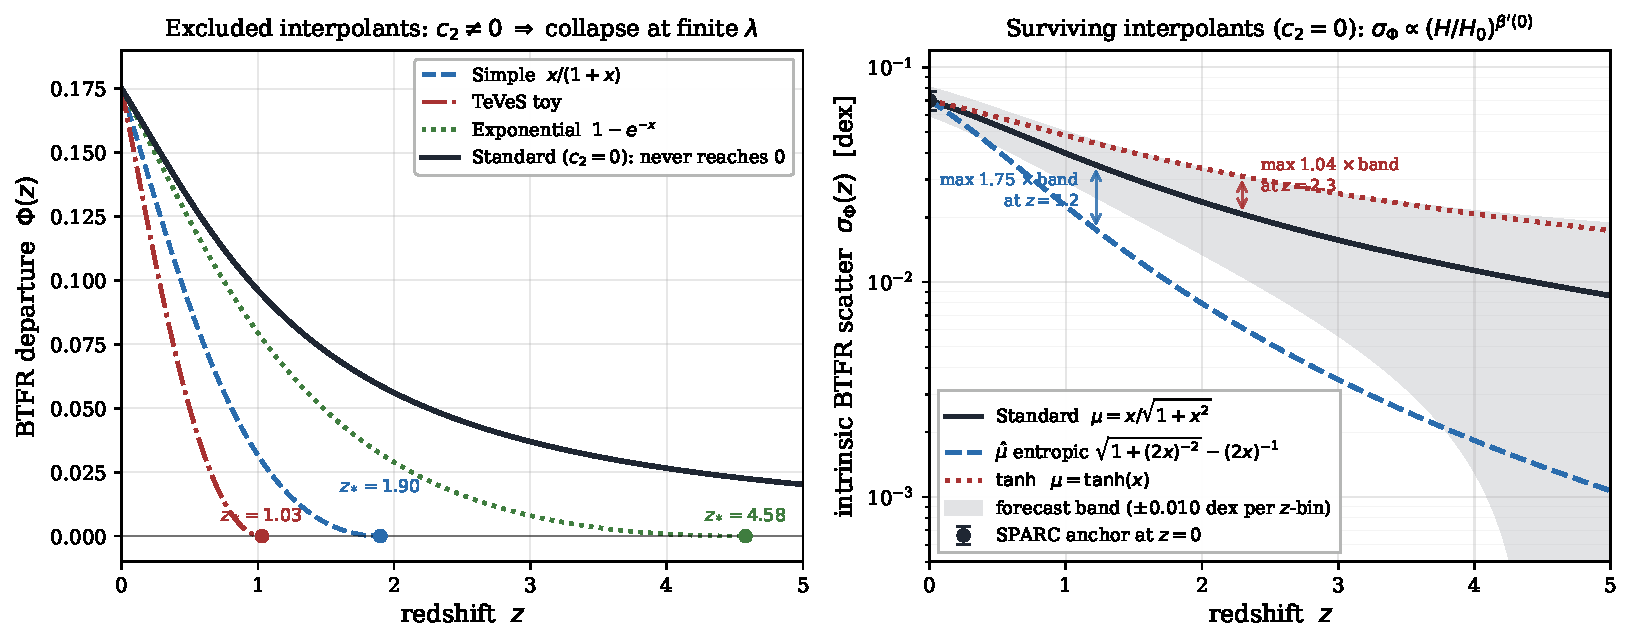
\includegraphics[width=\textwidth]{sigma_Phi_discriminator.pdf}
\caption{\emph{Left:} interpolating functions with $c_{2}\neq0$. The exact flow
$d\Phi/d\lambda=\beta(\Phi)$, integrated from $\Phi_{0}=0.175$ [Eq.~\eqref{eq:phi-zero}], drives the BTFR
departure to exactly zero at the finite flow times of
Table~\ref{tab:exclusion}, i.e.\ above the marked $z_{*}$; the standard
function ($c_{2}=0$, solid) relaxes exponentially and never reaches zero.
\emph{Right:} the three functions with $c_{2}=0$, whose intrinsic BTFR scatter
evolves as $\sigma_{\Phi}(z)=\sigma_{\Phi}(0)(H/H_{0})^{\beta'(0)}$
[Eq.~\eqref{eq:sigma-evolution}], against a forecast band of $\pm0.010$~dex per
redshift bin. Arrows mark the maximum separation from the standard prediction
in units of that band: $\hat\mu$ separates by at most $1.75$ band widths near
$z\simeq1.2$, $\tanh$ by at most $1.04$ near $z\simeq2.3$. Both curves are
computed in a flat $\Lambda$CDM background with $\Omega_{m}=0.3$ and
$\sigma_{\Phi}(0)=0.07$~dex.}
\label{fig:discriminator}
\end{figure}

\paragraph{From the allowed class to observables.} Within the surviving class
the flow is analytic, so each $\mu$ carries a definite slope and curvature, and
$\beta'(0)$ becomes an observational discriminator.
Under the flow, the intrinsic scatter about the BTFR evolves as
\begin{equation*}\tag{16}\label{eq:sigma-evolution}
\sigma_{\Phi}(z) \;=\; \sigma_{\Phi}(0)
   \left(\frac{H(z)}{H_{0}}\right)^{\beta'(0)},
\end{equation*}
which generalises~\eqref{eq:10}. Figure~\ref{fig:discriminator} shows the three
survivors together with a forecast band of $\pm0.010$~dex per redshift bin,
representative of a well-calibrated resolved-kinematics survey once
baryonic-mass systematics are controlled to $\sim0.05$~dex per galaxy. The
discriminating power is real but bounded, and we quantify it rather than assert
it: the separation between the standard function and $\hat\mu$ peaks at
$0.0175$~dex ($1.75$ times the forecast band) at $z\simeq1.2$, while the
separation between the standard function and $\tanh$ never exceeds
$0.0104$~dex ($1.04$ band widths, at $z\simeq2.2$). The separation does
\emph{not} grow monotonically with redshift: all surviving curves converge to
zero scatter, so the absolute difference --- the quantity a fixed error budget
must resolve --- is maximal at $z\simeq1$--$2$ and decreases thereafter. A
survey targeting this test should therefore concentrate on $z\simeq1$--$2$,
where $\hat\mu$ is separable from the standard form; distinguishing $\tanh$
requires a band narrower than the $\pm0.010$~dex assumed here.

\paragraph{Scope.} We emphasise the practical value of the criterion. Since
\eqref{eq:general-beta} follows from the flow equation~\eqref{eq:8} alone, and
uses neither Axioms~1--2 nor the theorem of \S\ref{sec:theorem}, the test
applies to any candidate interpolating function independently of whether the
axioms are adopted. Any theory whose galactic dynamics reduces to AQUAL, and
whose BTFR is required to be a linear attractor against cosmological expansion,
must supply a $\mu$ with $c_{2}=0$. This elevates the choice of interpolating
function from a phenomenological ansatz to a computable and observationally
testable condition.

Two boundaries are worth stating explicitly. First, the criterion applies
within the AQUAL flow structure of \S\ref{sec:corollaries}; theories whose BTFR
dynamics take a different form (non-attractor cycles, higher-derivative flows)
are not tested by~\eqref{eq:taylor}. Second, it probes only the deep-MOND
expansion: a candidate with $c_{2}=0$ can still be falsified at intermediate or
high $x$, where $c_{3},c_{4},\ldots$ enter observables sensitive to the
transition regime. The condition $c_{2}=0$ is necessary, not sufficient.

\section{Discussion}\label{sec:discussion}

\noindent\textbf{What is claimed.} (i) The standard MOND interpolating function is exactly the cumulative isotropic distribution of the projection ratio $\cot\theta$ --- equivalently, the solid-angle fraction under the tilt gate (Theorem, eqs.~\eqref{eq:3} and~\eqref{eq:5}); (ii) since the correspondence gate $\leftrightarrow$ $\mu$ is one-to-one, this entails a rigidity lemma --- any mechanism producing the standard $\mu$ through monotone angular gating must implement the tilt comparison (eq.~\eqref{eq:7}) --- while the selection content proper is the four-gate result plus the structural fact that only the $\alpha=2$ threshold variable is the projection ratio $\cot\theta$ (eqs.~\eqref{eq:6},~\eqref{eq:7prime}); (iii) the BTFR attractor structure ($\beta'(0)=-1$, $\kappa=1/2$) follows with no further input (eq.~\eqref{eq:9}).

\noindent\textbf{What is not claimed.} The theorem does not by itself derive MOND from first principles: it relocates the empirical content of $\mu$ into an activation rule and shows that rule to be geometrically distinguished. The dynamical origin of the tilt criterion (as a competition between a decoherence rate and a re-coherence rate, which also fixes the scale of $a_0$) is the subject of a forthcoming companion paper and is logically independent of the present result. The value of $a_0$ is an input here.

\noindent\textbf{Relation to previous work.} Derivations of an interpolating function from a physical mechanism do exist, and we state them precisely. Milgrom (1999) observed that the Unruh temperature excess of an accelerated observer in de Sitter space suggests $\hat\mu(x) = \sqrt{1+(2x)^{-2}} - (2x)^{-1}$; Klinkhamer \& Kopp (2011) and Klinkhamer (2012) obtained exactly that $\hat\mu$ --- together with the Bekenstein--Milgrom modified Poisson equation and $a_0 = 4\pi(c/\hbar)k_B T_{\min}$ --- from entropic gravity with a minimum temperature; Trippe (2013) obtained the simple function $x/(1+x)$ from a toy model of virtual massive gravitons; Pazy (2013) related $\mu$ to a ratio of holographic degrees of freedom without a closed form. Other frameworks obtain MOND-like behaviour without an interpolating function: emergent gravity yields $g_D=\sqrt{g_B a_0/6}$ [Verlinde 2017], superfluid dark matter postulates the MONDian phonon action $P(X)\propto X\sqrt{|X|}$ [Berezhiani \& Khoury 2015], and quantum-gravity arguments recover the scale $a_0$ and the deep-MOND regime with the transition left unspecified [Smolin 2017]. None of these derives the standard $\mu(x)=x/\sqrt{1+x^2}$, and none proceeds by counting directions: the mechanisms are thermodynamic or field-theoretic, not solid-angle geometry. The present result is therefore new on two specific counts: it is the standard function that emerges, and it emerges from isotropy alone. That the entropic route selects $\hat\mu$ while direction counting selects the standard $\mu$ makes the transition region of the radial-acceleration relation a potential observational discriminant between the two mechanisms.

\noindent\textbf{Falsifiability.} The construction is rigid: isotropy plus a hard tilt threshold give exactly $x/\sqrt{1+x^2}$, not a family. Data preferring a materially different $\mu$ (e.g., the simple function at high accelerations) would falsify the axioms as stated, or force a measurable anisotropy of the ensemble.

\section{Data availability}\label{sec:data}

All results are reproducible from the scripts archived with this letter. \texttt{verificacion\_letter.py} re-derives every numbered equation symbolically (sympy) and runs a $10^6$ Monte Carlo smoke test; the canonical derivations are \texttt{derivacion\_mu\_angulo\_solido\_gates\_direccionales.py} (the four gates of \S\ref{sec:uniqueness}, exact), \texttt{derivacion\_beta\_ensamble\_gates\_reduccion\_sympy.py} (the reduction of \S\ref{sec:corollaries}, exact via sympy), and \texttt{derivacion\_beta\_ensamble\_gates\_montecarlo\_estable.py} (the $10^7$ Monte Carlo of \S\ref{sec:corollaries}, verified to 50 digits with mpmath, with pre-declared acceptance bands and the anisotropic negative control; fixed seed). No proprietary data are used; the observational constraints cited are from the published SPARC literature. A record of the prior-literature search underlying the novelty claims of \S\ref{sec:discussion} is archived as \texttt{prior\_work\_verification.md}. The results of \S\ref{sec:general-criterion} and Appendix~\ref{app:audit} are reproduced by \texttt{audit\_theorem.py} (theorem, four gates, closed form, TeVeS identity, unit invariance and the general expansion), \texttt{flow\_coeffs.py} (the coefficients $c_2,c_3,\beta'(0),\kappa$ for each candidate $\mu$ and the numerical integration of the exact flow giving $z_*$), \texttt{final\_table.py} (which emits the \LaTeX{} of Table~1 directly from the computation, so the manuscript can be diffed against it rather than transcribed) and \texttt{make\_figure.py} (Figure~1). All are deterministic and run in under thirty seconds.

\noindent\textbf{Funding and competing interests.} This work received no external funding. The author declares no competing interests.

\section{References}\label{sec:refs}

\begin{itemize}[leftmargin=1.6em,itemsep=2pt]
\item Bekenstein, J.\ D.\ 2004, Phys.\ Rev.\ D 70, 083509 [\href{https://arxiv.org/abs/astro-ph/0403694}{arXiv:astro-ph/0403694}]; Erratum: Phys.\ Rev.\ D 71, 069901 (2005)
\item Bekenstein, J., Milgrom, M. 1984, ApJ 286, 7
\item Berezhiani, L., Khoury, J. 2015, Phys.\ Rev.\ D 92, 103510 [\href{https://arxiv.org/abs/1507.01019}{arXiv:1507.01019}]
\item Famaey, B., Binney, J.\ 2005, MNRAS 363, 603
\item Famaey, B., McGaugh, S. 2012, Living Rev.\ Relativ.\ 15, 10 [\href{https://arxiv.org/abs/1112.3960}{arXiv:1112.3960}]
\item Figueroa Torres, J.\ P.\ 2026, \emph{Lambda EG: Emergent Gravitational Coherence and Galactic Dynamics Without Particle Dark Matter}, Zenodo preprint, \href{https://doi.org/10.5281/zenodo.19784004}{doi:10.5281/zenodo.19784004}
\item Klinkhamer, F.\ R., Kopp, M.\ 2011, Mod.\ Phys.\ Lett.\ A 26, 2783 [\href{https://arxiv.org/abs/1104.2022}{arXiv:1104.2022}]
\item Klinkhamer, F.\ R.\ 2012, Mod.\ Phys.\ Lett.\ A 27, 1250056 [\href{https://arxiv.org/abs/1201.4160}{arXiv:1201.4160}]
\item Lelli, F., McGaugh, S., Schombert, J.\ 2016b, AJ 152, 157
\item McGaugh, S., Lelli, F., Schombert, J.\ 2016a, Phys.\ Rev.\ Lett.\ 117, 201101
\item Milgrom, M.\ 1983a, ApJ 270, 365; 1983b, ApJ 270, 371; 1983c, ApJ 270, 384
\item Milgrom, M.\ 1999, Phys.\ Lett.\ A 253, 273 [\href{https://arxiv.org/abs/astro-ph/9805346}{arXiv:astro-ph/9805346}]
\item Pazy, E.\ 2013, Phys.\ Rev.\ D 87, 084063 [\href{https://arxiv.org/abs/1302.4411}{arXiv:1302.4411}]
\item Smolin, L.\ 2017, Phys.\ Rev.\ D 96, 083523 [\href{https://arxiv.org/abs/1704.00780}{arXiv:1704.00780}]
\item Trippe, S.\ 2013, J.\ Korean Astron.\ Soc.\ 46, 41 [\href{https://arxiv.org/abs/1303.7071}{arXiv:1303.7071}]
\item Verlinde, E.\ 2017, SciPost Phys.\ 2, 016 [\href{https://arxiv.org/abs/1611.02269}{arXiv:1611.02269}]
\end{itemize}

\appendix

\section{Symbolic verification, general flow, and well-posedness}
\label{app:audit}

This appendix supplements the main text with (i) a symbolic verification of the
theorem of \S\ref{sec:theorem}, (ii) the gate--$\mu$ correspondence for the
interpolating functions of Table~\ref{tab:exclusion}, (iii) the derivation of
the general expansion~\eqref{eq:general-beta}, (iv) the invariance of the
criterion under the choice of acceleration unit, and (v) the well-posedness
analysis underlying~\eqref{eq:zstar}. All computations were carried out with
\texttt{sympy 1.14.0} and \texttt{scipy}, are deterministic, and are archived
with this letter as \verb|audit_theorem.py|, \verb|flow_coeffs.py|,
\verb|final_table.py|, and \verb|make_figure.py|.

\subsection{The theorem}

Under Axioms~1--2 the active fraction is
\begin{equation}
\mu(x) \;=\; \int_{\arctan(1/x)}^{\pi/2} \sin\theta\,d\theta
       \;=\; \cos\!\bigl(\arctan(1/x)\bigr)
       \;=\; \frac{x}{\sqrt{1+x^{2}}},
\label{app:mu-thm}
\end{equation}
with threshold density $\mu'(x)=(1+x^{2})^{-3/2}$ and Taylor expansion
$\mu(x)=x-\tfrac12x^{3}+\tfrac38x^{5}+\mathcal{O}(x^{7})$. In particular the
coefficient of $x^{2}$ vanishes identically --- the observation that seeds the
criterion of \S\ref{sec:general-criterion}.

\subsection{The four projection gates}

The classification of \S\ref{sec:uniqueness} is reproduced by direct
integration over the hemispherical measure:
\begin{center}
\small
\setlength{\tabcolsep}{4pt}
\begin{tabular}{llllc}
\toprule
Gate & Criterion & $\mu(x)$ & Both MOND limits & Analytic \\
\midrule
T (tilt)         & $g\sin\theta > a_0\cos\theta$ & $x/\sqrt{1+x^{2}}$
                 & yes & yes \\
M (magnitude)    & $g > a_0\cos\theta$ & $\min(x,1)$
                 & yes & no (kink at $x=1$) \\
L (longitudinal) & $g\cos\theta > a_0$
                 & $0$ if $x\le1$; $1-1/x$ if $x>1$
                 & no ($\mu\equiv0$ at low $x$) & no \\
P (perpendicular)& $g\sin\theta > a_0$
                 & $0$ if $x<1$; $\sqrt{1-1/x^{2}}$ if $x\ge1$
                 & no & no \\
\bottomrule
\end{tabular}
\end{center}
The magnitude gate M produces $\mu_{M}-x\mu_{M}'\equiv0$ on $x<1$, whence the
flow function vanishes identically and the BTFR does not attract, as
anticipated in \S\ref{sec:uniqueness}.

\subsection{Gate--$\mu$ correspondence for published interpolating functions}

The bijection lemma associates every monotone $\mu(x)$ with a unique monotone
gate $f(\theta)=\mu^{-1}(\cos\theta)$:
\begin{center}
\begin{tabular}{lll}
\toprule
$\mu(x)$ & Corresponding gate $f(\theta)$ & Structure \\
\midrule
$x/\sqrt{1+x^{2}}$ & $\cot\theta$
   & longitudinal/transverse projection ratio \\
$x/(1+x)$ & $\cos\theta/(1-\cos\theta)$ & not a projection ratio \\
$\sqrt{1+(2x)^{-2}}-(2x)^{-1}$ & $\cos\theta/\sin^{2}\!\theta$
   & not a two-projection ratio \\
$2x/(1+2x+\sqrt{1+4x})$ & $\cos\theta/(1-\cos\theta)^{2}$
   & not a projection ratio \\
$1-e^{-x}$ & $-\ln(1-\cos\theta)$ & transcendental \\
$\tanh x$ & $\operatorname{arctanh}(\cos\theta)$ & transcendental \\
\bottomrule
\end{tabular}
\end{center}
Within the empirical family $\mu_{\alpha}(x)=x/(1+x^{\alpha})^{1/\alpha}$ the
gate is $f_{\alpha}(\theta)=\cos\theta/(1-\cos^{\alpha}\theta)^{1/\alpha}$,
reducing to $\cot\theta$ if and only if $\alpha=2$, which confirms
identity~\eqref{eq:7prime}. The TeVeS toy function is quoted here in the form
$2x/(1+2x+\sqrt{1+4x})$; it is algebraically identical to the published form
$(\sqrt{1+4x}-1)/(\sqrt{1+4x}+1)$ of Bekenstein (2004), as verified
symbolically in \verb|audit_theorem.py|.

\subsection{Derivation of the general expansion of \texorpdfstring{$\beta(\Phi)$}{beta(Phi)}}
\label{app:general-derivation}

Consider a monotone interpolating function with the expansion
\begin{equation}
\mu(u) \;=\; u + c_{2}u^{2} + c_{3}u^{3} + \mathcal{O}(u^{4}),
\qquad
\mu'(u) \;=\; 1 + 2c_{2}u + 3c_{3}u^{2} + \mathcal{O}(u^{3}).
\label{app:mu-expansion}
\end{equation}
The numerator of the flow function~\eqref{eq:8} expands as
\begin{equation}
\mu - u\mu' \;=\; -c_{2}u^{2} - 2c_{3}u^{3} + \mathcal{O}(u^{4}),
\label{app:numerator}
\end{equation}
and, using $\mu+u\mu' = 2u + 3c_{2}u^{2} + 4c_{3}u^{3} + \mathcal{O}(u^{4})$,
\begin{equation}
\mu(\mu+u\mu') \;=\; 2u^{2} + 5c_{2}u^{3}
                   + \bigl(3c_{2}^{2}+6c_{3}\bigr)u^{4} + \mathcal{O}(u^{5}).
\label{app:denominator}
\end{equation}
Hence
\begin{equation}
\beta(u) \;=\; -\frac{u(\mu-u\mu')}{\mu(\mu+u\mu')}
       \;=\; \frac{c_{2}}{2}\,u
             + \Bigl(c_{3}-\frac{5c_{2}^{2}}{4}\Bigr)u^{2}
             + \mathcal{O}(u^{3}).
\label{app:beta-u}
\end{equation}
Changing variable to $\Phi=\sqrt{1+u^{2}}-1$, so that $u^{2}=\Phi(2+\Phi)$ and
near $\Phi=0$
\begin{equation}
u=\sqrt{2\Phi}\bigl(1+\tfrac14\Phi+\mathcal{O}(\Phi^{2})\bigr),
\qquad
u^{2}=2\Phi+\Phi^{2}+\mathcal{O}(\Phi^{3}),
\label{app:u-of-Phi}
\end{equation}
and substituting into~\eqref{app:beta-u} through $\mathcal{O}(\Phi)$ gives
Eq.~\eqref{eq:general-beta} of the main text,
\begin{equation}
\beta(\Phi) \;=\; \frac{c_{2}}{\sqrt2}\sqrt{\Phi}
                 + 2\Bigl(c_{3}-\frac{5c_{2}^{2}}{4}\Bigr)\Phi
                 + \mathcal{O}(\Phi^{3/2}).
\label{app:general-beta-derived}
\end{equation}
If $c_{2}=0$ this reduces to $\beta(\Phi)=2c_{3}\Phi+\mathcal{O}(\Phi^{2})$, so
that $\beta'(0)=2c_{3}$ is fixed by the cubic coefficient
of~\eqref{app:mu-expansion}. For the standard form $c_{3}=-1/2$, giving
$\beta'(0)=-1$ as in \S\ref{sec:corollaries}. Note that the linear term of
$\beta$ depends on $c_{3}$ for every $\mu$: the coincidence
$2(c_{3}-\tfrac54c_{2}^{2})=-1$ for the standard function is a property of that
function, not a general identity.

\subsection{Invariance under the choice of acceleration unit}
\label{app:invariance}

The coefficients in~\eqref{app:mu-expansion} are defined relative to an
acceleration unit, and the framework paper uses $g_{\mathrm{crit}}=a_{0}/4\pi$
rather than $a_{0}$; it must therefore be checked that the criterion is not an
artefact of that choice. Under $u\to su$ with the deep-MOND normalisation
restored, $\mu_{s}(u)\equiv\mu(su)/s = u + sc_{2}u^{2} + s^{2}c_{3}u^{3}+\dots$,
so
\begin{equation}
c_{2}\longmapsto s\,c_{2},
\qquad
c_{3}\longmapsto s^{2}c_{3}.
\label{app:scaling}
\end{equation}
The value of $c_{2}$ is therefore convention-dependent, but its vanishing is
not: $c_{2}=0\Leftrightarrow sc_{2}=0$ for any $s>0$. The criterion of
\S\ref{sec:general-criterion} is thus invariant under any rescaling of the
acceleration unit. The derived quantities $\beta'(0)=2c_{3}$ and $\kappa$ are
moreover unambiguous, because the transformation~\eqref{app:scaling} does not
preserve the Newtonian limit --- $\mu_{s}(\infty)=1/s$ --- so requiring both
MOND limits fixes $s=1$ uniquely.

\subsection{Well-posedness of the flow and the origin of \texorpdfstring{$z_{*}$}{z*}}
\label{app:wellposedness}

For $c_{2}\neq0$ the leading behaviour $\beta\simeq(c_{2}/\sqrt2)\sqrt{\Phi}$
is continuous but not Lipschitz at $\Phi=0$, since
$d\beta/d\Phi\sim\Phi^{-1/2}\to\infty$. Two standard consequences follow.

\emph{Non-uniqueness.} The Picard--Lindel\"of theorem does not apply. Writing
$a=c_{2}/\sqrt2<0$, both $\Phi\equiv0$ and
\begin{equation}
\Phi(\lambda)=\frac{a^{2}}{4}\,(\lambda-\lambda_{*})^{2},
\qquad \lambda\le\lambda_{*},
\label{app:peano}
\end{equation}
solve $d\Phi/d\lambda=a\sqrt{\Phi}$ with the same data at $\lambda_{*}$; only
the Peano existence theorem survives. The renormalisation-group flow therefore
loses uniqueness at the fixed point.

\emph{Finite-time collapse.} Integrating from $\Phi(0)=\Phi_{0}$ gives
$2\sqrt{\Phi}=2\sqrt{\Phi_{0}}+a\lambda$, so $\Phi$ reaches zero at
\begin{equation}
\lambda_{*}=\frac{2\sqrt{2\Phi_{0}}}{|c_{2}|},
\label{app:lambda-star}
\end{equation}
a \emph{finite} flow time, rather than approaching it asymptotically. We stress
that this corrects a natural misreading: the $c_{2}\neq0$ branch does not
relax more slowly than the exponential case, it relaxes faster, reaching the
fixed point exactly. What fails is linearity --- and with it, the standard
interpretation of $\beta'(0)$ as a relaxation rate --- not attraction.

Since $\lambda=\ln(H/H_{0})$ increases towards the past, \eqref{app:lambda-star}
implies that the intrinsic BTFR scatter vanishes identically for
$z>z_{*}$, where $H(z_{*})/H_{0}=e^{\lambda_{*}}$. Values of $z_{*}$ quoted in
Table~\ref{tab:exclusion} are obtained by numerical integration of the
\emph{exact} flow~\eqref{eq:8} rather than from~\eqref{app:lambda-star}, which
uses only the leading term; for $\sigma_{\Phi}(0)=0.07$~dex and
$\Omega_{m}=0.3$ the two agree to better than $14\%$ ($\lambda_{*}=1.040$
exact versus $1.183$ leading-order, for the simple function).

\subsection{Positivity of \texorpdfstring{$\Phi$}{Phi} and the delta component at the fixed point}
\label{app:delta-component}

The identity~\eqref{eq:phi-identity} follows from AQUAL directly. With
$g=V^{2}/R$, $g_{N}=G\bar M/R^{2}$ and $u_{0}=g/a_{0}$, the field equation
$\mu(u_{0})\,g=g_{N}$ gives $R^{2}=G\bar M/[\mu(u_{0})g]$, whence
\begin{equation}
\frac{V^{4}}{G\bar M a_{0}}
 \;=\; \frac{g^{2}R^{2}}{G\bar M a_{0}}
 \;=\; \frac{u_{0}}{\mu(u_{0})}
 \;=\; \sqrt{1+u_{0}^{2}}
\label{app:phi-identity}
\end{equation}
for the standard $\mu$. Hence $\Phi=\sqrt{1+u_{0}^{2}}-1\ge0$, with equality
only at $u_{0}=0$. The dynamical departure is one-sided: transition-regime
galaxies lie above the asymptotic BTFR. Observational residuals about a fitted
BTFR are of either sign and include mass-calibration systematics; they are a
different quantity and the criterion does not apply to them.

The positivity is what makes a delta component at $\Phi=0$ meaningful, and the following
elementary statement makes it diagnostic.

\medskip
\noindent\textbf{Proposition.} \emph{Let $\beta$ be continuous with
$\beta(0)=0$ and let $\Phi_{0}>0$. If $\beta$ is Lipschitz on a neighbourhood
of $0$, no trajectory reaches $\Phi=0$ in finite flow time.}

\smallskip
\noindent\emph{Proof.} Lipschitz continuity with $\beta(0)=0$ gives
$|\beta(\Phi)|\le L\Phi$ near the origin, so $d\Phi/d\lambda\ge-L\Phi$ and
Gr\"onwall's inequality yields $\Phi(\lambda)\ge\Phi_{0}e^{-L\lambda}>0$ for all
finite $\lambda$. $\square$

\smallskip
Conversely, for $\beta\simeq(c_{2}/\sqrt2)\sqrt{\Phi}$ with $c_{2}<0$ the
collapse time~\eqref{app:lambda-star} is finite and \emph{increasing} in
$\Phi_{0}$. A population with a spread of departures therefore separates: at
each $\lambda$ some members sit exactly at $\Phi=0$ while the rest have not yet
arrived, and the distribution of $\Phi$ acquires a delta component (a Dirac mass
at the origin) of
growing weight. Combining the two directions,
\begin{equation}
\text{a delta component at } \Phi=0 \text{ forms}
\iff
\beta \text{ is not Lipschitz at the fixed point.}
\label{app:iff}
\end{equation}
The signature is thus tied to the analytic structure of the flow rather than to
any particular $\mu$, and cannot be reproduced by reparametrising a Lipschitz
flow. It requires one ingredient beyond the flow --- that the population carry a
spread of $\Phi$ --- which is the same premise already underlying
Eq.~\eqref{eq:10}. The distribution's shape is not predicted and sets only the
rate at which the delta component accumulates.

\subsection{Numerical verification of the flow (no series expansion)}
\label{app:numerics}

As an independent check that the dichotomy is not an artefact of truncating a
series, the exact equation $d\Phi/d\lambda=\beta(\Phi)$, with $\beta$
evaluated from~\eqref{eq:8} without expansion, was integrated numerically from
$\Phi_{0}=0.175$ with an adaptive solver (\texttt{scipy}, relative tolerance
$10^{-11}$) and a terminal event at $\Phi=10^{-9}$:
\begin{center}
\begin{tabular}{lccc}
\toprule
$\mu(x)$ & $c_{2}$ & $\Phi(\lambda=1)$ & $\lambda_{*}$ \\
\midrule
Standard $x/\sqrt{1+x^{2}}$ & $0$ & $6.13\times10^{-2}$ & --- \\
$\hat\mu$ entropic          & $0$ & $2.83\times10^{-2}$ & --- \\
$\tanh x$                   & $0$ & $8.33\times10^{-2}$ & --- \\
Simple $x/(1+x)$            & $-1$ & $2.05\times10^{-4}$ & $1.040$ \\
TeVeS toy                   & $-2$ & $0$ & $0.583$ \\
Exponential $1-e^{-x}$      & $-1/2$ & $3.53\times10^{-2}$ & $1.983$ \\
\bottomrule
\end{tabular}
\end{center}
The $c_{2}=0$ cases remain strictly positive for all $\lambda$ (exponential
relaxation); the $c_{2}\neq0$ cases terminate at finite $\lambda_{*}$, as
predicted.

\subsection{Taylor coefficients}

For completeness, the intermediate coefficients entering
Table~\ref{tab:exclusion}, verified symbolically:
\begin{center}
\begin{tabular}{lcccc}
\toprule
$\mu(x)$ & $c_{2}$ & $c_{3}$ & $\beta'(0)$ (if $c_{2}=0$) & $\kappa$ \\
\midrule
$x/\sqrt{1+x^{2}}$             & $0$    & $-1/2$ & $-1$   & $+1/2$ \\
$\sqrt{1+(2x)^{-2}}-(2x)^{-1}$ & $0$    & $-1$   & $-2$   & $-3$   \\
$\tanh x$                      & $0$    & $-1/3$ & $-2/3$ & $+3/5$ \\
$x/(1+x)$                      & $-1$   & $+1$   & ---    & ---    \\
$2x/(1+2x+\sqrt{1+4x})$        & $-2$   & $+5$   & ---    & ---    \\
$1-e^{-x}$                     & $-1/2$ & $+1/6$ & ---    & ---    \\
\bottomrule
\end{tabular}
\end{center}
Here $\kappa$ is defined by $\beta(\Phi)=\beta'(0)\Phi-\kappa\Phi^{2}
+\mathcal{O}(\Phi^{3})$, consistently with \S\ref{sec:corollaries}. The members
$\mu_{\alpha}$ with $\alpha\ge3$ have $c_{2}=c_{3}=0$, giving the degenerate
case $\beta'(0)=0$ in which the linear term vanishes and the approach to the
fixed point is set by subleading terms; they are included only to show that
smoothness of $\mu$ alone does not guarantee a non-degenerate linear attractor.

\subsection{Reproducibility}

The scripts \verb|audit_theorem.py|, \verb|flow_coeffs.py|,
\verb|final_table.py|, and \verb|make_figure.py| perform, respectively:
(i) symbolic verification of~\eqref{app:mu-thm}, the four-gate classification,
the closed form~\eqref{eq:9}, and the TeVeS identity; (ii) the expansion of
$\beta$ for each candidate $\mu$, the change of variable to $\Phi$ with correct
handling of half-integer powers, and the numerical integration of
\S\ref{app:numerics}; (iii) compilation of the tables; and (iv) generation of
Figure~\ref{fig:discriminator}. All are deterministic (no Monte Carlo) and
execute in under thirty seconds on a standard workstation.

\end{document}
